%%%%%%%%%%%%%%%%%%%%%%%%%%%%%%%%%%%%%%%%%%%%%%%%%%%%%%%%%%%%%%%%%%%%%%
%%%%%%%%% Select one of the options, and comment the rest of them

%%%%%%%%%% Option 1:  to compile with pdflatex : parameter "t" - to align to the top
\documentclass[professionalfonts,t]{beamer}
%sans font?

%%%%%%%%%% Option 3: to create handout for print
%\documentclass[t,handout]{beamer}
%\usepackage{pgfpages}              % to put several slides on one page
%\pgfpagesuselayout{2 on 1}[a4paper, border shrink=5mm]             % 2 slides on 1 page
%\pgfpagesuselayout{4 on 1}[a4paper,landscape, border shrink=5mm]   % 4 slides on 1 page, and landscaped


%%%%%%%%%%%%%%%%%%%%%%%%%%%%%%%%%%%%%%%%%%%%%%%%%%%%%%%%%%%%%%%%%%%%
%%%%%%%%%%%%%% Select the Theme %%%%%%%%%%%%%%%%%%%%%%%%%%%%%%%%%%%
\usetheme{Dresden}     % OK
%\usetheme{Berlin}
%\usetheme{Bergen}      % NO
%\usetheme{Boadilla}    % NO
%\usetheme{Copenhagen}  % NO
%\usetheme{Hannover}    % NO
%\usetheme{Luebeck}     % NO
%\usetheme{Marburg}     % NO
%\usetheme{Pittsburgh}  % NO
%\usetheme{default}
%\usetheme{Singapore}   % OK
%\usetheme{boxes}
%\usecolortheme{structure}
%\usecolortheme{rose}
%\usecolortheme{beaver}


\definecolor{mymaroon}{cmyk}{0.0, 1.0, 1.0, 0.498}
\definecolor{myblue}{cmyk}{1.0, 1, 0, 0.5}
\definecolor{mygreen}{cmyk}{100, 0, 100, 50}
\setbeamercolor*{palette secondary}{use=structure,fg=white,bg=myblue}
\setbeamercolor*{palette tertiary}{use=structure,fg=white,bg=mymaroon}

%\usepackage{beamerthemesplit}              %
\beamertemplateballitem % fancy bullets and numbering

\setbeamertemplate{navigation symbols}{}   % suppress navigation symbols
\addtobeamertemplate{frametitle}{}{%
	\logo{../../images/IIT_logo}
	\iffalse
	
	\begin{tikzpicture}[remember picture,overlay]
	\node[anchor=center, yshift=-13pt, xshift=-5pt] at (current page.north) 
	{\includegraphics[height=1.1cm]{../images/Argonne_cmyk_black-eps-converted-to}\hspace{10cm}};
	
	\node[anchor=north east, yshift=3pt, xshift=0pt] at (current page.north east) 
	{\includegraphics[height=0.7cm]{../images/IIT_Logo_blk}};
	\end{tikzpicture}
    
     \fi
}
% other possibilities to include LOGO. it puts it in RLC

%
%\pgfdeclareimage[width=1cm]{logo}{../images/IIT_Logo}
%\logo{\pgfuseimage{logo}}


% load additional packages

\usepackage{xcolor}
\usepackage{graphicx}
\usepackage{amsmath}
\usepackage{amssymb}
\usepackage{amsthm}
\usepackage{graphicx}
\usepackage{url}
\usepackage{color}
\usepackage{booktabs} % Allows the use of \toprule, \midrule and \bottomrule in tables
\usepackage{pifont}% http://ctan.org/pkg/pifont
\usepackage{epstopdf}
\usepackage[export]{adjustbox}
\usepackage{tikz}
\usetikzlibrary{shapes.misc}
\usetikzlibrary{shapes,arrows,decorations.markings,shadows,positioning}

% Your Abbreviations
\newcommand\bE{{\mathbb{E}}}
\newcommand\bR{{\mathbb{R}}}
\newcommand\bH{{\mathbf{H}}}
% End abbreviations

\newcommand\Wider[2][3em]{%
	\makebox[\linewidth][c]{%
		\begin{minipage}{\dimexpr\textwidth+#1\relax}
			\raggedright#2
		\end{minipage}%
	}%\textbf{}
}

%%%%%%%%%%%%%%%%%%%%% to edit the main text below
%NOTES ON SOME TECHNICS
%%%% Box %%%%%%%%%%%%%%%%%%%%%%%%%%%%%%%%%%%%%%%%%%%%%%%
%{\fbox{ \parbox[t]{10cm}{ SOME TEXT }}}

%%% include a picture. The file should be with extention EPS, e.g. FILENAME.EPS
%\begin{figure}[h]
%\centering
%\includegraphics[width=.7\linewidth]{FILENAME}
%\caption{{\footnotesize PUT_CAPTION }}
%\end{figure}

%\subtitle{}
%\institute[ANL/IIT]{Argonne National Laboratory\\Illinois Institute of Technology}

\title[June 2018]{Simulations, Optimization, and Experimental Measurements at the AWA}
\author[N.Neveu]{{\Large Nicole Neveu}}
\institute[ANL, IIT] % (optional, but mostly needed)
{   Illinois Institute of Technology \\
	Argonne National Laboratory \\
    \url{nneveu@anl.gov} 
}
% - Use the \inst command only if there are several affiliations.
% - Keep it simple, no one is interested in your street address.
\date{ \today \\
\includegraphics[width=3cm,keepaspectratio]{/home/nicole/Documents/presentations/logos/Argonne_cmyk_black}%
\hfill \hfill \hfill%
\includegraphics[width=4cm,keepaspectratio]{/home/nicole/Documents/presentations/logos/IIT_Logo_blk-eps-converted-to}%
}

%\date[IIT, April 2009]{
%           Space Charge 2017 \\ Oc 18, 2009  }

%%%%%%%%%%%%%%%%%%%%%%%%%%%%%%Section title frame 
\AtBeginSection[]{
	\begin{frame}
	\vfill
	\centering
	
	\begin{minipage}{0.55\textwidth}
		%\begin{beamercolorbox}[sep=8pt,center,shadow=true,rounded=true]{title}
		\tableofcontents[currentsection]
		%\usebeamerfont{title}\insertsectionhead\par%
		%\end{beamercolorbox}	
	\end{minipage}\hfill
	\begin{minipage}{0.35\textwidth}
		\includegraphics[width=4cm]{\secimage}
		
		%Source: Fermilab Media
	\end{minipage}
	%\vfill 
\end{frame}
}
%%%%%%%%%%%%%%%%%%%%%%%%%%%%%%Section title frame

\newcommand{\secimage}{/home/nicole/Pictures/misc/hough_transform}


\begin{document}


\begin{frame}
  \titlepage
\end{frame}

\begin{frame}
	\frametitle{Outline}
	\tableofcontents
\end{frame}

\section{Facility Intro and Simulations}
%\subsection{AWA Facility Introduction}
\begin{frame}
\frametitle{Argonne Wakefield Accelerator Facility (AWA)}
\Wider[4em]{
	\setlength{\leftmargin}{0.1cm}	
	%\begin{minipage}{0.6\textwidth}
		\begin{itemize}
			\item{Two photocathode guns and linacs}
			\begin{itemize}
				\item{\underline{\textbf{Drive Line}}: $Cs_2Te$ cathode, 6 linac cavities}
				\begin{itemize}
					\item{Charge 0.1-100nC}
					\item{Energy up to 70 MeV}
					
				\end{itemize}
				\item{\underline{\textbf{Witness Line}}: $Mg$ cathode, 1 linac cavity}
				\begin{itemize}
					\item{Charge 0.1-10nC}
					\item{Energy up to 15 MeV}
				\end{itemize}
			\end{itemize}
		\end{itemize}	
	%\end{minipage}
	%\begin{minipage}{0.35\textwidth}
	%\vspace{0.5em}
		\centering
		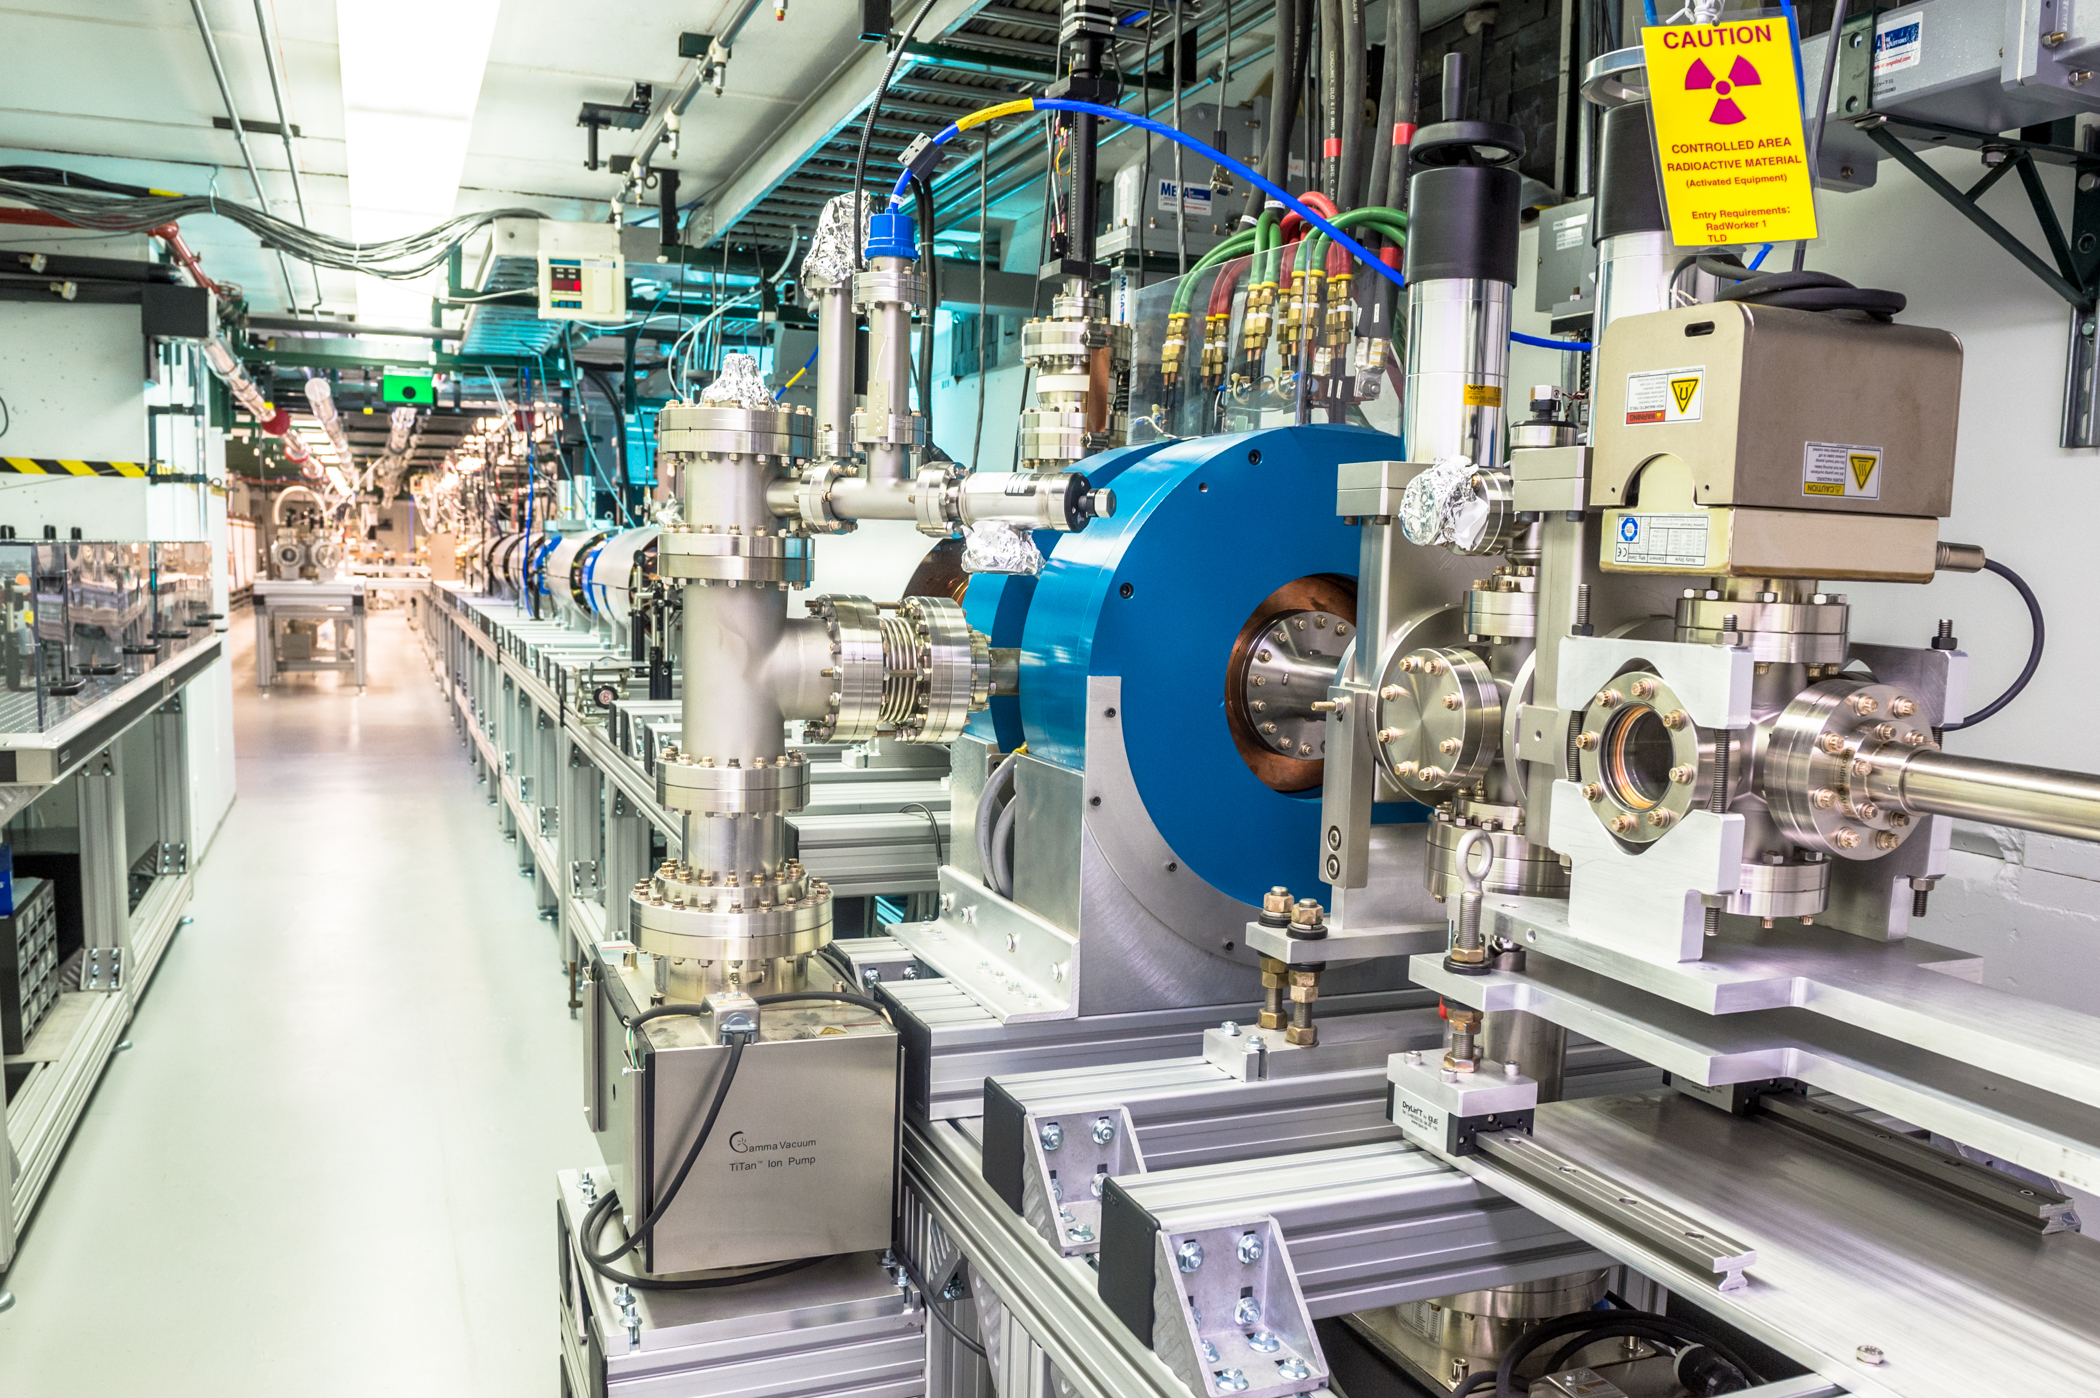
\includegraphics[width=0.45\linewidth]{/home/nicole/Documents/presentations/space_charge_2017/drive_gun}
	%\end{minipage}
}
\end{frame}


\begin{frame}
\frametitle{AWA Facility}
Current experiments include:
\begin{itemize}
	\item{Two Beam Acceleration (TBA)}
	\item{Dielectric accelerating and decelerating structure tests}
	\item{Beam line design for TBA = my thesis}
\end{itemize}
\vspace{0.5cm}
\includegraphics[width=0.49\linewidth]{/home/nicole/Documents/presentations/space_charge_2017/stage}\hfill\includegraphics[width=0.49\linewidth]{/home/nicole/Documents/presentations/space_charge_2017/dielectrics}

\end{frame}

\begin{frame}
\frametitle{AWA Facility}
Current experiments include:
\begin{itemize}
\item{Emittance Exchange (EEX)}
\item{Electron Radiography Imaging (ERI)}
\item{Cathode Studies}
\item Plasma wakefield (very recent)
\end{itemize}
\vspace{0.3cm}
\centering
\includegraphics[width=0.65\linewidth]{/home/nicole/Documents/presentations/space_charge_2017/EEX}
\end{frame}

\subsection{Layout}
\begin{frame}
\frametitle{Drive Line Layout}
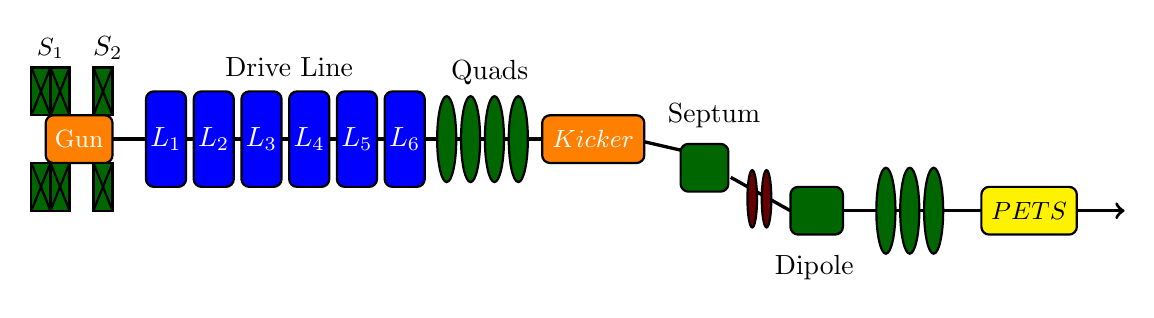
\begin{tikzpicture}[scale=\textwidth/20cm, text=black]
%\begin{tikzpicture}[scale=0.5, text=black]
\def \gunleft {-1.0}
\def \gunright {0.3}
\def \loneright {1.0}
\def \ltworight {2.0}
\def \lthreeright {3.0}
\def \lfourright {4.0}
\def \lfiveright {5.0}
\def \lsixright {6.0}
\def \quadone {7.3}
\def \quadfour{16}

\draw[very thick, ->] (0.0,1) -- (10,1);

\draw[fill=orange, thick, rounded corners =0.1cm] (\gunleft-0.1,0.5)rectangle (\gunright,1.5) node[pos=.5, white] {\small{Gun}} ;
%Straight through

%S1
\node[] at (-1,2.9) {\small{$S_1$}};
\draw[thick, fill=black!60!green] (-1.4,-0.5)rectangle  (-1.0,0.5) node[pos=.5, white] {} ;
\draw[black,  thick] (-1.4,-0.5) -- (-1.0,0.5);
\draw[black,  thick] (-1.4,0.5) -- (-1.0,-0.5);
\draw[ thick, fill=black!60!green] (-1.4,1.5)rectangle  (-1.0,2.5) node[pos=.5, white] {} ;
\draw[black,  thick] (-1.4,1.5) -- (-1.0,2.5);
\draw[black,  thick] (-1.4,2.5) -- (-1.0,1.5);

\draw[ thick, fill=black!60!green] (-1.0,-0.5)rectangle  (-0.6,0.5) node[pos=.5, white] {} ;
\draw[black,  thick] (-1.0,-0.5) -- (-0.6,0.5);
\draw[black,  thick] (-1.0,0.5) -- (-0.6,-0.5);
\draw[ thick, fill=black!60!green] (-1.0,1.5)rectangle  (-0.6,2.5) node[pos=.5, white] {} ;
\draw[black,  thick] (-1.0,1.5) -- (-0.6,2.5);
\draw[black,  thick] (-1.0,2.5) -- (-0.6,1.5);

%S2
\node[] at (0.2,2.9) {$S_2$};
\draw[ thick, fill=black!60!green] (-0.1,-0.5) rectangle  (0.3,0.5) node[pos=.5, white] {};
\draw[black,  thick] (-0.1,-0.5) -- (0.3,0.5);
\draw[black,  thick] (-0.1,0.5) -- (0.3,-0.5);
\draw[ thick, fill=black!60!green] (-0.1,1.5) rectangle  (0.3,2.5) node[pos=.5, white] {};
\draw[black,  thick] (-0.1,1.5) -- (0.3,2.5);
\draw[black,  thick] (-0.1,2.5) -- (0.3,1.5);
%Linac drawings 
%\node[] at (4,2.5) {Accelerating Cavities};
\draw[fill=blue,  thick, rounded corners =0.1cm] (\loneright,0)rectangle  ({\loneright+0.84},2) node[pos=.5, white] {$L_1$} ;
\draw[fill=blue,  thick, rounded corners =0.1cm] (\ltworight,0)rectangle  ({\ltworight+0.84},2) node[pos=.5, white] {$L_2$};
\draw[fill=blue,  thick, rounded corners =0.1cm] (\lthreeright,0)rectangle ({\lthreeright+0.84},2) node[pos=.5, white] {$L_3$};
\draw[fill=blue,  thick, rounded corners =0.1cm] (\lfourright,0)rectangle ({\lfourright+0.84},2) node[pos=.5, white] {$L_4$};
\draw[fill=blue,  thick, rounded corners =0.1cm] (\lfiveright,0)rectangle ({\lfiveright+0.84},2) node[pos=.5, white] {$L_5$};
\draw[fill=blue,  thick, rounded corners =0.1cm] (\lsixright,0)rectangle ({\lsixright+0.84},2) node[pos=.5, white] {$L_6$};



%Quad drawings
\node[] at (8.2,2.4) {Quads};
\draw[fill=black!60!green,  thick] (\quadone, 1.0) ellipse (0.2cm and 0.9cm);
\draw[fill=black!60!green,  thick] (\quadone+0.5, 1.0) ellipse (0.2cm and 0.9cm);
\draw[fill=black!60!green,  thick] (\quadone+1.0, 1.0) ellipse (0.2cm and 0.9cm);
\draw[fill=black!60!green,  thick] (\quadone+1.5, 1.0) ellipse (0.2cm and 0.9cm);

%Line between kicker and septum
\node[] at (4,2.5) {Drive Line};
\draw[very thick] (\lsixright+5.2,1.0) -- (12.5,0.7);

%Kicker 
\draw[fill=orange,  thick, rounded corners =0.1cm] (\lsixright+3.3,0.5)rectangle ({\lsixright+0.84+4.6},1.5) node[pos=.5, white] {\small{$Kicker$}};

%Septum
\node[] at (12.9,1.5) {Septum};
\draw[fill=black!60!green,  thick, rounded corners =0.1cm] (12.2,0.9)rectangle ({13.2},-0.1) node[pos=.5, white] {};
%\draw[latex-latex] (\gunleft,-5.0) -- (14,-5.0) ;
%\foreach \x in  {0.3, 1.0, 3.5, 5.0, 7.0, 8.5, 10, 12.5} %tick marks
%\draw[shift={(\x,-5.0)},color=black] (0pt,3pt) -- (0pt,-3pt);
%\foreach \x in {0.3, 1.0, 3.5, 5.0, 7.0, 8.5, 10, 12.5}
%\draw[shift={(\x,-5.2)},color=black] (0pt,0pt) node[below] {$\x$};

%Line between kicker and septum
\draw[very thick] (13.25,0.2) -- (14.5,-0.5);

%Second set of quads
\draw[fill=black!60!red,  thick] (\quadfour-2.3, -0.250) ellipse (0.1cm and 0.6cm);
\draw[fill=black!60!red,  thick] (\quadfour-2, -0.250) ellipse (0.1cm and 0.6cm);

%Dipole
\node[] at (15,-1.7) {Dipole};
\draw[fill=black!60!green, thick, rounded corners =0.1cm] (14.5,0.0)rectangle ({15.6},-1.0) node[pos=.5, white] {};

%Line between dipole and quads
\draw[very thick, ->] (15.6,-0.5) -- (21.5,-0.5);
%Second set of quads
\draw[fill=black!60!green,  thick] (\quadfour+0.5, -0.50) ellipse (0.2cm and 0.9cm);
\draw[fill=black!60!green,  thick] (\quadfour+1.0, -0.50) ellipse (0.2cm and 0.9cm);
\draw[fill=black!60!green,  thick] (\quadfour+1.5, -0.50) ellipse (0.2cm and 0.9cm);

%Kicker 
\draw[fill=yellow,  thick, rounded corners =0.1cm] (\quadfour+2.5,0)rectangle ({\quadfour+4.5},-1) node[pos=.5, black] {\small{$PETS$}};






\end{tikzpicture}

%\vspace{3em}
For the remainder of the talk, I will focus on simulation and experimental results for the beam line above.

\vspace{1em}

Main PIC Code of Choice: OPAL

\vspace{1em}

Limited experience with G4beamline, Elegant, and IMPACT.

\end{frame}

\begin{frame}
\frametitle{Benchmark: ASTRA, GPT, OPAL-t}
\begin{itemize}
	\item{Motivated by code features and my inexperience}
	\item{Used RF and solenoid maps from AWA photocathode gun}
	\begin{itemize}
		\item 2D SUPERFISH/POISSON
		\item 3D CST MWS and ACE3P (future/current work)
	\end{itemize}
	\item{Used PITZ operating conditions as input parameters}
	\item{Poster presented at NAPAC'16: THPOA46}
	\item{Spoiler: No major differences found at 1 nC}
	\begin{itemize}
		\item However, a lot of work to match input parameters
	\end{itemize}
\end{itemize}
\end{frame}


\begin{frame}
\frametitle{Model and Input Parameters}
\begin{minipage}{0.3\textwidth}
	\def \gunleft {-1.0}
	\def \gunright {0.3}
	\def \loneright {1.0}
	\def \ltworight {3.5}
	\def \lthreeright {5.0}
	\def \lfourright {7.0}
	\def \lfiveright {8.5}
	\def \lsixright {10}
	\begin{center}
		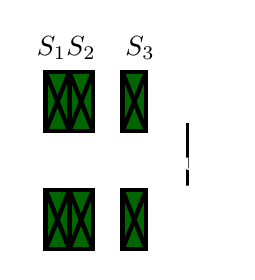
\begin{tikzpicture}[scale=0.75]
		%Gun drawings
		\draw[fill=orange, very thick, rounded corners =0.1cm] (\gunleft,0.5)rectangle (\gunright,1.5) node[pos=.5, white] {\textbf{Gun}} ;
		
		%S1
		\node[] at (-1.3,2.9) {$S_1$};
		\draw[ultra thick, fill=black!60!green] (-1.4,-0.5)rectangle  (-1.0,0.5) node[pos=.5, white] {} ;
		\draw[black, ultra thick] (-1.4,-0.5) -- (-1.0,0.5);
		\draw[black, ultra thick] (-1.4,0.5) -- (-1.0,-0.5);
		\draw[ultra thick, fill=black!60!green] (-1.4,1.5)rectangle  (-1.0,2.5) node[pos=.5, white] {} ;
		\draw[black, ultra thick] (-1.4,1.5) -- (-1.0,2.5);
		\draw[black, ultra thick] (-1.4,2.5) -- (-1.0,1.5);
		%S2
		\node[] at (-0.8,2.9) {$S_2$};
		\draw[ultra thick, fill=black!60!green] (-1.0,-0.5)rectangle  (-0.6,0.5) node[pos=.5, white] {} ;
		\draw[black, ultra thick] (-1.0,-0.5) -- (-0.6,0.5);
		\draw[black, ultra thick] (-1.0,0.5) -- (-0.6,-0.5);
		\draw[ultra thick, fill=black!60!green] (-1.0,1.5)rectangle  (-0.6,2.5) node[pos=.5, white] {} ;
		\draw[black, ultra thick] (-1.0,1.5) -- (-0.6,2.5);
		\draw[black, ultra thick] (-1.0,2.5) -- (-0.6,1.5);
		
		%S3
		\node[] at (0.2,2.9) {$S_3$};
		\draw[ultra thick, fill=black!60!green] (-0.1,-0.5) rectangle  (0.3,0.5) node[pos=.5, white] {};
		\draw[black, ultra thick] (-0.1,-0.5) -- (0.3,0.5);
		\draw[black, ultra thick] (-0.1,0.5) -- (0.3,-0.5);
		\draw[ultra thick, fill=black!60!green] (-0.1,1.5) rectangle  (0.3,2.5) node[pos=.5, white] {};
		\draw[black, ultra thick] (-0.1,1.5) -- (0.3,2.5);
		\draw[black, ultra thick] (-0.1,2.5) -- (0.3,1.5);
		\end{tikzpicture}
	\end{center}
\end{minipage} \hfill
\begin{minipage}{0.65\textwidth}
	\begin{table}\centering
		\begin{tabular}{l c c}
			\toprule 
			\textbf{Parameter} & \textbf{Value} \\
			\midrule
			Charge  		& 1 nC \\
			$S_3$ 			&  -0.389 T \\
			$S_1$ and $S_2$ & -0.12 T \\
			Laser Radius 	& 0.75 mm \\
			Laser FWHM 		& 20 ps \\
			Laser Rise/Fall Time & 6 ps \\
			Gun Gradient 	& 60 MV/m \\
			Phase 			& Max Energy \\
			Kinetic Energy on Cathode & 0.55 eV \\
			\bottomrule
		\end{tabular}
	\end{table}
\end{minipage}
\end{frame}


\begin{frame}
\frametitle{Benchmark Results}
\Wider[4em]{
All codes matched within $5\%$. \\
Well below measurement thresholds at AWA.\\  
\vskip12pt
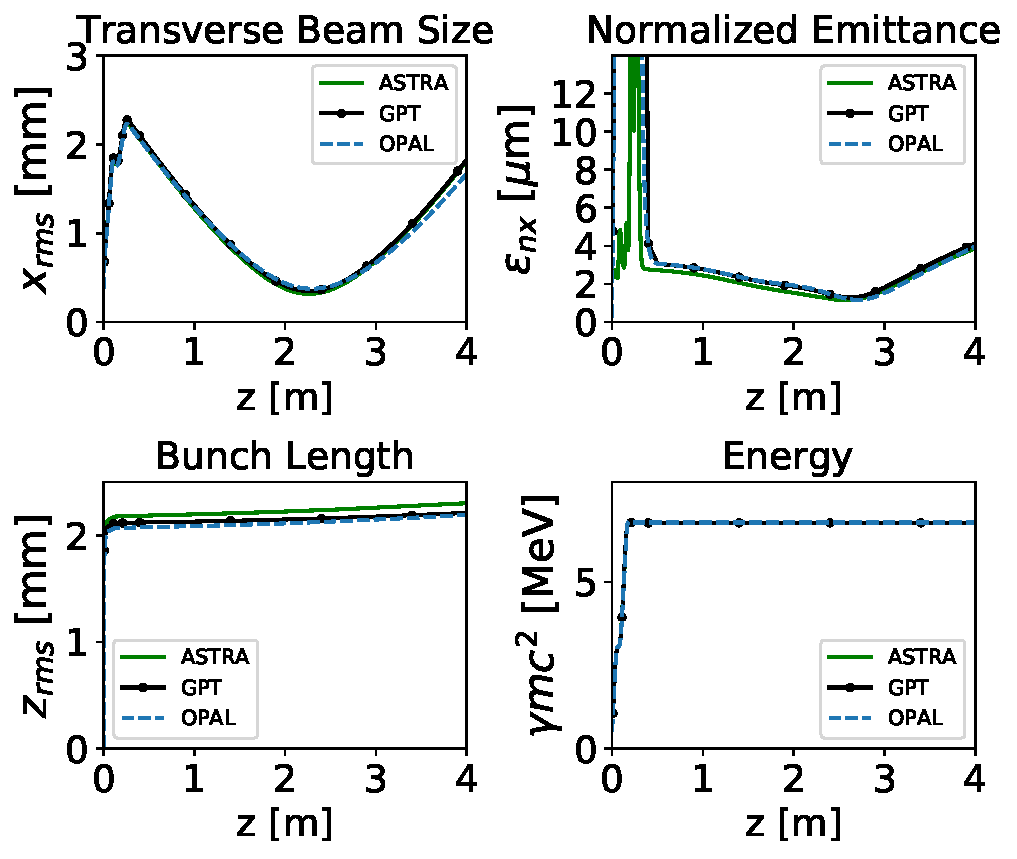
\includegraphics[width=0.49\linewidth]{/home/nicole/Documents/thesis/tex/images/benchmark_5m}\hfill 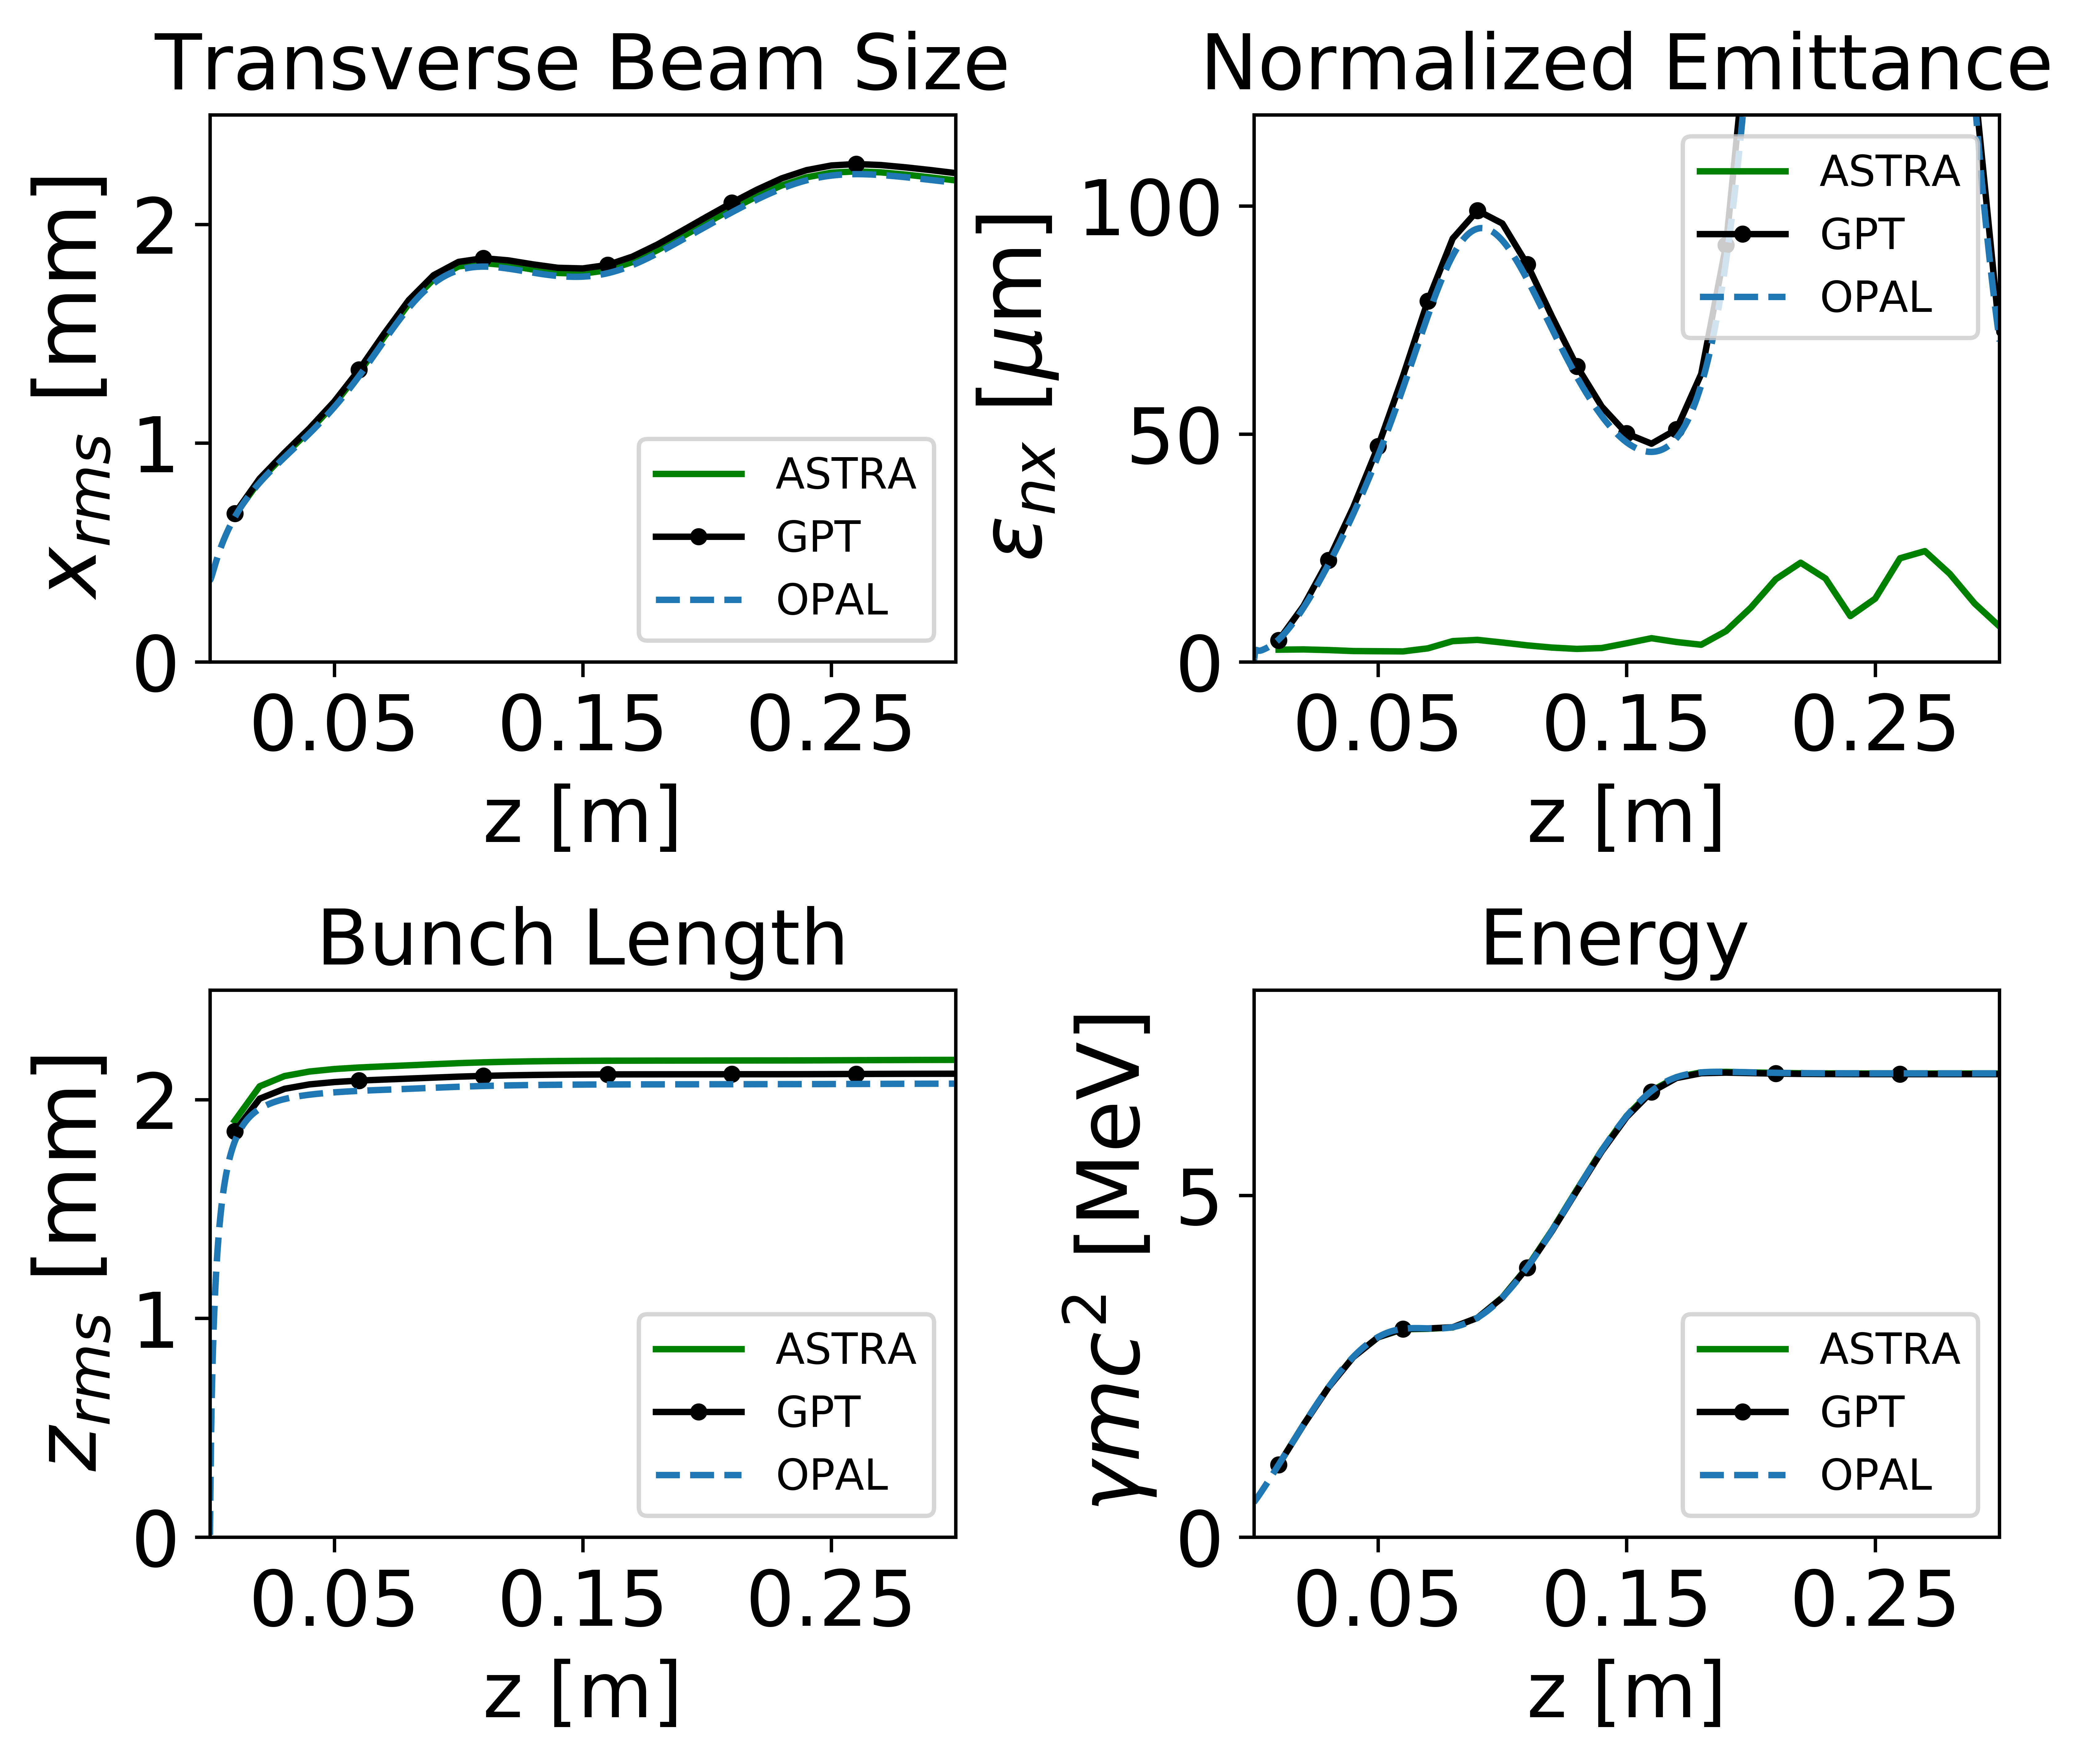
\includegraphics[width=0.49\linewidth]{/home/nicole/Documents/thesis/tex/images/benchmark_gun}
}
\end{frame}

\section{Linac Optimization}
\subsection{Model Based Algorithm}
\begin{frame}
\frametitle{Linac Optimization: Code Used}
\begin{itemize}
	\setlength\itemsep{2em}
	\item Used python library NLopt: \url{http://ab-initio.mit.edu/wiki/index.php/Main_Page}
	
	\item Code summary can be found at: \url{http://www.mcs.anl.gov/~jlarson/AWA}
	
	\item Complete repo at: \url{git@xgitlab.cels.anl.gov:jmlarson/emittance_minimization.git}
\end{itemize}	
\end{frame}

\begin{frame}
\frametitle{Optimization using scalarization (Linac only)}
\Wider[4em]{
\begin{minipage}{0.6\textwidth}
	\begin{itemize}
		\item{Determine what emittance and bunch length we can expect from the linac}
		\begin{itemize}
			\item{Understand beam at entrance of quads}
			\item After $L_6$: $z_1=12.51$ m
		\end{itemize}
		\item{Used algorithm BOBYQA from NLopt}
		\item{Varied 10 parameters:}
	\end{itemize}
\end{minipage}%
\begin{minipage}{0.4\textwidth}
	\def \gunleft {-1.0}
	\def \gunright {0.3}
	\def \loneright {1.0}
	\def \ltworight {2.0}
	\def \lthreeright {3.0}
	\def \lfourright {4.0}
	\def \lfiveright {5.0}
	\def \lsixright {6.0}
	\centering
	\begin{center}
		\begin{tikzpicture}[scale=0.55]%,use optics
		%Gun drawings
		\draw[fill=orange, very thick, rounded corners =0.1cm] (\gunleft-0.2,0.5)rectangle (\gunright,1.5) node[pos=.5, white] {\textbf{Gun}} ;
		
		%S1
		\node[] at (-1.5,2.9) {$S_1$};
		\draw[ultra thick, fill=black!60!green] (-1.4,-0.5)rectangle  (-1.0,0.5) node[pos=.5, white] {} ;
		\draw[black, ultra thick] (-1.4,-0.5) -- (-1.0,0.5);
		\draw[black, ultra thick] (-1.4,0.5) -- (-1.0,-0.5);
		\draw[ultra thick, fill=black!60!green] (-1.4,1.5)rectangle  (-1.0,2.5) node[pos=.5, white] {} ;
		\draw[black, ultra thick] (-1.4,1.5) -- (-1.0,2.5);
		\draw[black, ultra thick] (-1.4,2.5) -- (-1.0,1.5);
		%S2
		\node[] at (-0.8,2.9) {$S_2$};
		\draw[ultra thick, fill=black!60!green] (-1.0,-0.5)rectangle  (-0.6,0.5) node[pos=.5, white] {} ;
		\draw[black, ultra thick] (-1.0,-0.5) -- (-0.6,0.5);
		\draw[black, ultra thick] (-1.0,0.5) -- (-0.6,-0.5);
		\draw[ultra thick, fill=black!60!green] (-1.0,1.5)rectangle  (-0.6,2.5) node[pos=.5, white] {} ;
		\draw[black, ultra thick] (-1.0,1.5) -- (-0.6,2.5);
		\draw[black, ultra thick] (-1.0,2.5) -- (-0.6,1.5);
		
		%S3
		\node[] at (0.2,2.9) {$S_3$};
		\draw[ultra thick, fill=black!60!green] (-0.1,-0.5) rectangle  (0.3,0.5) node[pos=.5, white] {};
		\draw[black, ultra thick] (-0.1,-0.5) -- (0.3,0.5);
		\draw[black, ultra thick] (-0.1,0.5) -- (0.3,-0.5);
		\draw[ultra thick, fill=black!60!green] (-0.1,1.5) rectangle  (0.3,2.5) node[pos=.5, white] {};
		\draw[black, ultra thick] (-0.1,1.5) -- (0.3,2.5);
		\draw[black, ultra thick] (-0.1,2.5) -- (0.3,1.5);
		%Linac drawings 
		\draw[fill=blue, ultra thick, rounded corners =0.1cm] (\loneright,0)rectangle  ({\loneright+0.84},2) node[pos=.5, white] {$L_1$} ;
		\draw[fill=blue, ultra thick, rounded corners =0.1cm] (\ltworight,0)rectangle  ({\ltworight+0.84},2) node[pos=.5, white] {$L_2$};
		\draw[fill=blue, ultra thick, rounded corners =0.1cm] (\lthreeright,0)rectangle ({\lthreeright+0.84},2) node[pos=.5, white] {$L_3$};
		\draw[fill=blue, ultra thick, rounded corners =0.1cm] (\lfourright,0)rectangle ({\lfourright+0.84},2) node[pos=.5, white] {$L_4$};
		\draw[fill=blue, ultra thick, rounded corners =0.1cm] (\lfiveright,0)rectangle ({\lfiveright+0.84},2) node[pos=.5, white] {$L_5$};
		\draw[fill=blue, ultra thick, rounded corners =0.1cm] (\lsixright,0)rectangle ({\lsixright+0.84},2) node[pos=.5, white] {$L_6$};
		\end{tikzpicture}
	\end{center}
\end{minipage}%
\begin{center}
	\setcounter{mpfootnote}{\value{footnote}}%
	\renewcommand{\thempfootnote}{\arabic{mpfootnote}}%	
	\begin{tabular}{ l *{3}{c}}
		%\toprule
		\textbf{Variable} & \textbf{Range} & \textbf{Unit} \\
		\midrule
		Solenoid Strength & $ 0 \le S_3 \le 440$  & amps \\
		Phase of Gun & $-60 \le \phi_g \le 60$  & degrees \\
		Laser Radius  & $0.1 \le R \le 30$  & mm \\
		Laser FWHM  & $2 \le T \le $10  & ps \\
		Cavity Phase & $-20 \le \phi_L \le 20$\footnote[1]{$\phi_L=[\phi_{L_1},\ldots,\phi_{L_6}]$} & degrees
		%\bottomrule    
	\end{tabular}
\end{center}
}
\end{frame}

\begin{frame}
\frametitle{Linac Optimization}
\begin{itemize}
\item{1,000 point sample was done}
\item{132 simulations completed w/o error}
\item{Scaled and shifted raw values to remove unit dependence}
\end{itemize}
\begin{align*}
\bar{\epsilon}_x (v,z_1) = \frac{ \epsilon_x (v,z_1) - \epsilon_{\min} } { \epsilon_{\max} - \epsilon_{\min} }
\end{align*}

\begin{itemize}
\item{Used 11 weights from 0-1}
\item{Solved 11 optimization problems $f(v,w)$ using BOBYQA}
\end{itemize}
\begin{gather*}
w\in\left\{ 0, \,0.1, \,0.2, \ldots, 1 \right\}\\ \\
f(v,w) = w \,\bar{\epsilon}_x(v,z_1) + (1-w)\, \bar{\sigma}_z(v,z_1)
\end{gather*}


\end{frame}

\begin{frame}
\frametitle{BOBYQA Results}
Progress during each BOBYQA run:
\centering
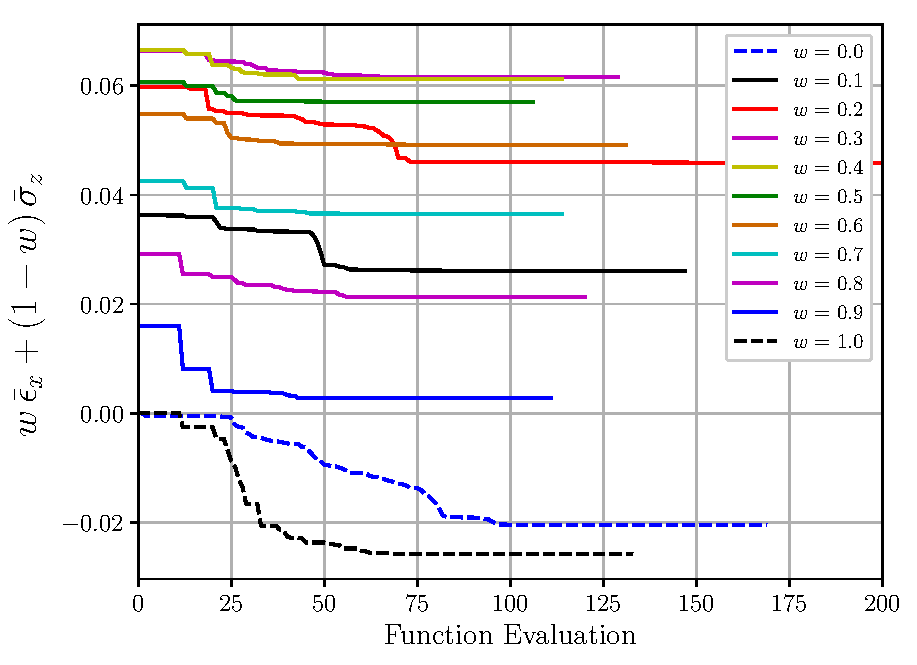
\includegraphics[width=0.75\textwidth]{/home/nicole/Documents/thesis/tex/images/THPAB155f2}
\end{frame}

\begin{frame}
\frametitle{Approximate Pareto Front}
\centering
Trade off between emittance and bunch length
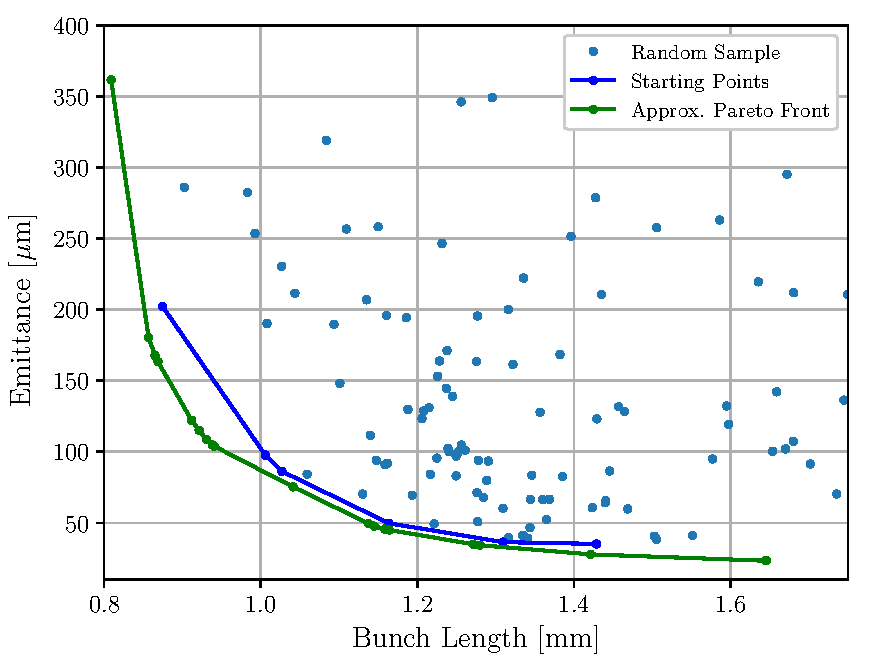
\includegraphics[width=0.7\textwidth]{/home/nicole/Documents/thesis/tex/images/THPAB155f1}
\begin{itemize}
\item In total, 2,492 simulations made this plot.
\end{itemize}
\end{frame}

\begin{frame}
\frametitle{Beam line under design}
\Wider[4em]{
\def \gunleft {-1.0}
\def \gunright {0.3}
\def \loneright {1.0}
\def \ltworight {2.0}
\def \lthreeright {3.0}
\def \lfourright {4.0}
\def \lfiveright {5.0}
\def \lsixright {6.0}
\def \quadone {7.5}
\centering
\begin{center}
\begin{tikzpicture}[scale=0.6]%,use optics
%Gun drawings
\draw[fill=orange, very thick, rounded corners =0.1cm] (\gunleft,0.5)rectangle (\gunright,1.5) node[pos=.5, white] {\textbf{Gun}} ;

%S1
\node[] at (-1.3,2.9) {$S_1$};
\draw[ultra thick, fill=black!60!green] (-1.4,-0.5)rectangle  (-1.0,0.5) node[pos=.5, white] {} ;
\draw[black, ultra thick] (-1.4,-0.5) -- (-1.0,0.5);
\draw[black, ultra thick] (-1.4,0.5) -- (-1.0,-0.5);
\draw[ultra thick, fill=black!60!green] (-1.4,1.5)rectangle  (-1.0,2.5) node[pos=.5, white] {} ;
\draw[black, ultra thick] (-1.4,1.5) -- (-1.0,2.5);
\draw[black, ultra thick] (-1.4,2.5) -- (-1.0,1.5);
%S2
\node[] at (-0.8,2.9) {$S_2$};
\draw[ultra thick, fill=black!60!green] (-1.0,-0.5)rectangle  (-0.6,0.5) node[pos=.5, white] {} ;
\draw[black, ultra thick] (-1.0,-0.5) -- (-0.6,0.5);
\draw[black, ultra thick] (-1.0,0.5) -- (-0.6,-0.5);
\draw[ultra thick, fill=black!60!green] (-1.0,1.5)rectangle  (-0.6,2.5) node[pos=.5, white] {} ;
\draw[black, ultra thick] (-1.0,1.5) -- (-0.6,2.5);
\draw[black, ultra thick] (-1.0,2.5) -- (-0.6,1.5);

%S3
\node[] at (0.2,2.9) {$S_3$};
\draw[ultra thick, fill=black!60!green] (-0.1,-0.5) rectangle  (0.3,0.5) node[pos=.5, white] {};
\draw[black, ultra thick] (-0.1,-0.5) -- (0.3,0.5);
\draw[black, ultra thick] (-0.1,0.5) -- (0.3,-0.5);
\draw[ultra thick, fill=black!60!green] (-0.1,1.5) rectangle  (0.3,2.5) node[pos=.5, white] {};
\draw[black, ultra thick] (-0.1,1.5) -- (0.3,2.5);
\draw[black, ultra thick] (-0.1,2.5) -- (0.3,1.5);
%Linac drawings 
\draw[fill=blue, ultra thick, rounded corners =0.1cm] (\loneright,0)rectangle  ({\loneright+0.84},2) node[pos=.5, white] {$L_1$} ;
\draw[fill=blue, ultra thick, rounded corners =0.1cm] (\ltworight,0)rectangle  ({\ltworight+0.84},2) node[pos=.5, white] {$L_2$};
\draw[fill=blue, ultra thick, rounded corners =0.1cm] (\lthreeright,0)rectangle ({\lthreeright+0.84},2) node[pos=.5, white] {$L_3$};
\draw[fill=blue, ultra thick, rounded corners =0.1cm] (\lfourright,0)rectangle ({\lfourright+0.84},2) node[pos=.5, white] {$L_4$};
\draw[fill=blue, ultra thick, rounded corners =0.1cm] (\lfiveright,0)rectangle ({\lfiveright+0.84},2) node[pos=.5, white] {$L_5$};
\draw[fill=blue, ultra thick, rounded corners =0.1cm] (\lsixright,0)rectangle ({\lsixright+0.84},2) node[pos=.5, white] {$L_6$};

%current optimization point
%\node[draw, fill=yellow, star, star points=5, star point ratio=0.6, minimum size=0.1cm]
%at (12.5,1.0) {$z_1$};


%Quad drawings
\draw[fill=black!60!green] (\quadone, 1.0) ellipse (0.2cm and 0.9cm);
\draw[fill=black!60!green] (\quadone+0.5, 1.0) ellipse (0.2cm and 0.9cm);
\draw[fill=black!60!green] (\quadone+1.0, 1.0) ellipse (0.2cm and 0.9cm);
\draw[fill=black!60!green] (\quadone+1.5, 1.0) ellipse (0.2cm and 0.9cm);

%Line between kicker and septum
\draw[very thick] (\lsixright+5.3,1.0) -- (12.5,0.7);

%Kicker 
\draw[fill=orange, ultra thick, rounded corners =0.1cm] (\lsixright+3.5,0.5)rectangle ({\lsixright+0.84+4.6},1.5) node[pos=.5, white] {$Kicker$};

%Septum
\node[] at (12.7,1.5) {Septum};
\draw[fill=black!60!green, ultra thick, rounded corners =0.1cm] (12.2,0.9)rectangle ({13.2},-0.1) node[pos=.5, white] {};
%\draw[latex-latex] (\gunleft,-5.0) -- (14,-5.0) ;
%\foreach \x in  {0.3, 1.0, 3.5, 5.0, 7.0, 8.5, 10, 12.5} %tick marks
%\draw[shift={(\x,-5.0)},color=black] (0pt,3pt) -- (0pt,-3pt);
%\foreach \x in {0.3, 1.0, 3.5, 5.0, 7.0, 8.5, 10, 12.5}
%\draw[shift={(\x,-5.2)},color=black] (0pt,0pt) node[below] {$\x$};

%Line between kicker and septum
\draw[very thick] (13.25,0.2) -- (14.5,-0.5);

%Dipole
\node[] at (15,-1.7) {Dipole};
\draw[fill=black!60!green, ultra thick, rounded corners =0.1cm] (14.5,0.0)rectangle ({15.6},-1.0) node[pos=.5, white] {};

%Line between septum and dipole
\draw[very thick] (15.6,-0.5) -- (16.5,-0.5);
\end{tikzpicture}
\end{center}

}


Possible Optimization Parameters:
\begin{itemize}
\item Four-six quads 
\item Distance between quads and septum
\item Distance between kicker and septum
\item Distance between septum and dipole
\item Plus, 10 variables in gun and linac 
\end{itemize}
\end{frame}

\subsection{Genetic Algorithms}
\begin{frame}
\frametitle{Genetic Algorithm Work}

\begin{itemize}
	\item Starting with piece wise approach
	\item Use brute force optimization to investigate parameter space.
\end{itemize}

\vspace{0.5em}
Given information above, does a nominal solution exist that will satisfy tba requirements for this non-ideal situation. With the requirements being:
\begin{itemize}
	\item 100\% transmission 
	\begin{itemize}
		\item good beam size at structure
		\item good emittance at structure
	\end{itemize}
	\item Reasonable bunch length at structure
	\begin{itemize}
		\item to maximize power generated
	\end{itemize}
\end{itemize}
\end{frame}

\begin{frame}
\frametitle{Optimization Objectives}
Objectives are beam parameters the simulation tries to minimize.
These points are picked to improve beam parameters at key locations, 
i.e. the PETS structure.

\vspace{1em}
\begin{minipage}{0.45\textwidth}
	\begin{table}[hbt] 
		\centering
		\begin{tabular}{ l *{3}{c}}
			\toprule
			\textbf{Variable} &  \textbf{Unit} \\
			\midrule
			$\sigma_z$ 		& mm \\
			$\sigma_{x}$ 	& mm \\
			$\sigma_y$ 		& mm \\
			$\sigma_{px}$ 	& mm-mrad \\
			$\sigma_{py}$ 	& mm-mrad \\
			$dE$			& MeV\\
			\bottomrule	
		\end{tabular}	
	\end{table}
\end{minipage}
\begin{minipage}{0.45\textwidth}
	\begin{itemize}
		\item 3 optimized locations ($z_k$, $z_s$, $z_d$)
		\item 18 Objectives
		\item 10 variables 
		\item 6 Constraints
	\end{itemize}
\end{minipage}
\centering
Note, these take an extremely large time to simulate (order days).
\end{frame}


%%%%%%%%%%%%%%%%%%%%%%%%%%%%%%%%%%%%%%%%%%%%%%%%%%%%%%%%%%%%%%%%%%%%%%%%%%%%%%%%
\begin{frame}
\frametitle{PETS}
Reminder: form factor and bunch length are related. PETS aperture = 17.6 mm

\begin{minipage}{0.49\textwidth}
\includegraphics[width=\textwidth]{/home/nicole/Documents/awa-tba/whole_line/rms_z}
\end{minipage}
\begin{minipage}{0.49\textwidth}

\centering
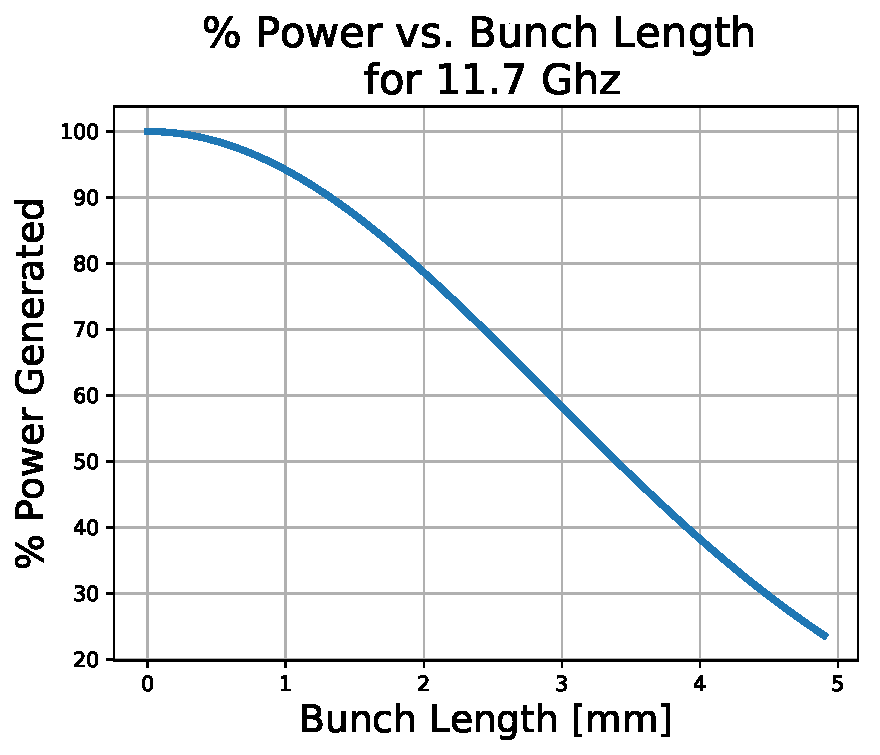
\includegraphics[width=\textwidth]{/home/nicole/Documents/thesis_code/formfactorsqrd}
\end{minipage}
\end{frame}


\section{Experimental Measurements}
\subsection{Beam Size and Energy Measurements}

\begin{frame}
\frametitle{Energy Measurments}
\end{frame}

\begin{frame}
\frametitle{Beam Sizes}
YAG screen images 
\end{frame}

\begin{frame}
	Beam size along beam line
\end{frame}


\subsection{Solenoid Scans and Bunch Length}
\begin{frame}[t]
\frametitle{Matching Solenoid Scans}
\begin{columns}[T]
	\begin{column}{0.76\textwidth}
		\begin{minipage}{0.5\textheight}
			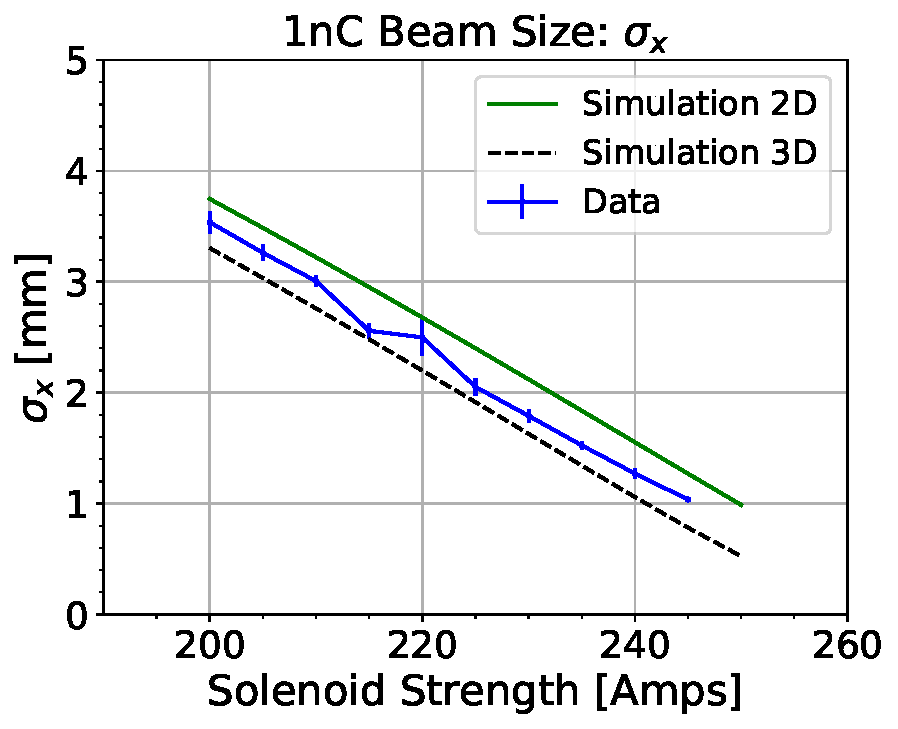
\includegraphics[width=1.0\linewidth]{/home/nicole/Documents/presentations/group_meetings/xbeamsizes_low_charge_sol_scan_11-02-2017}	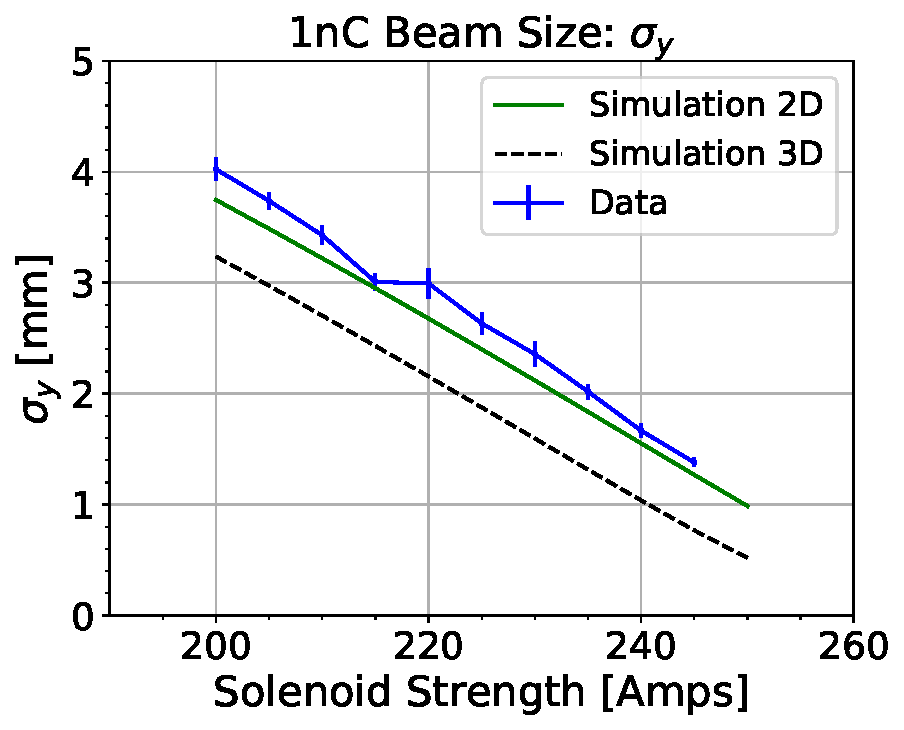
\includegraphics[width=1.0\linewidth]{/home/nicole/Documents/presentations/group_meetings/ybeamsizes_low_charge_sol_scan_11-02-2017}
		\end{minipage}
		\begin{minipage}{0.5\textheight}
			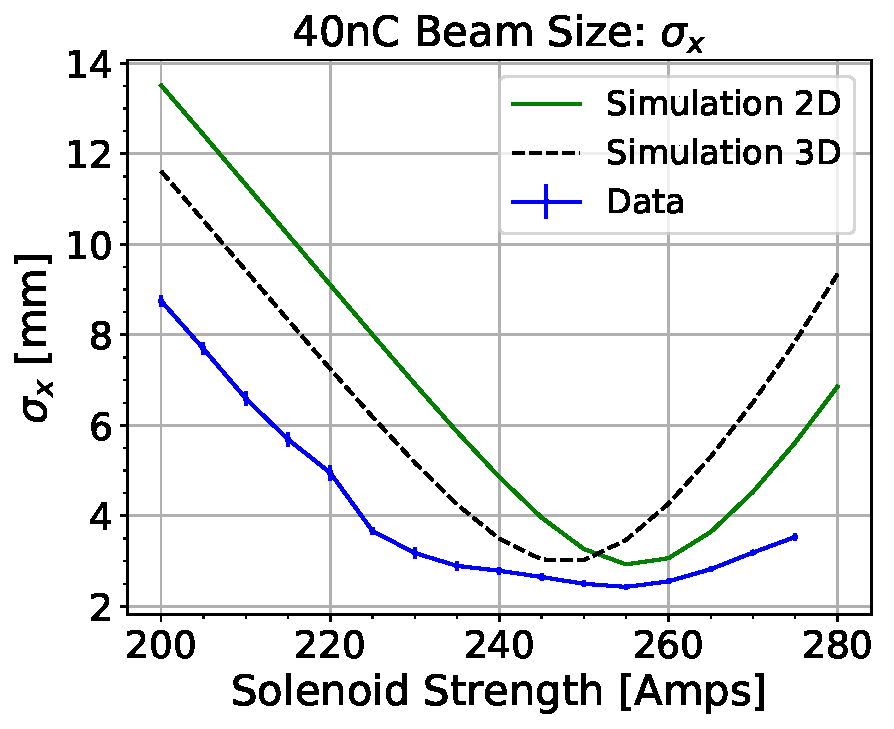
\includegraphics[width=1.0\linewidth]{/home/nicole/Documents/presentations/group_meetings/xbeamsizes_high_charge_sol_scan_10-17-2017}
			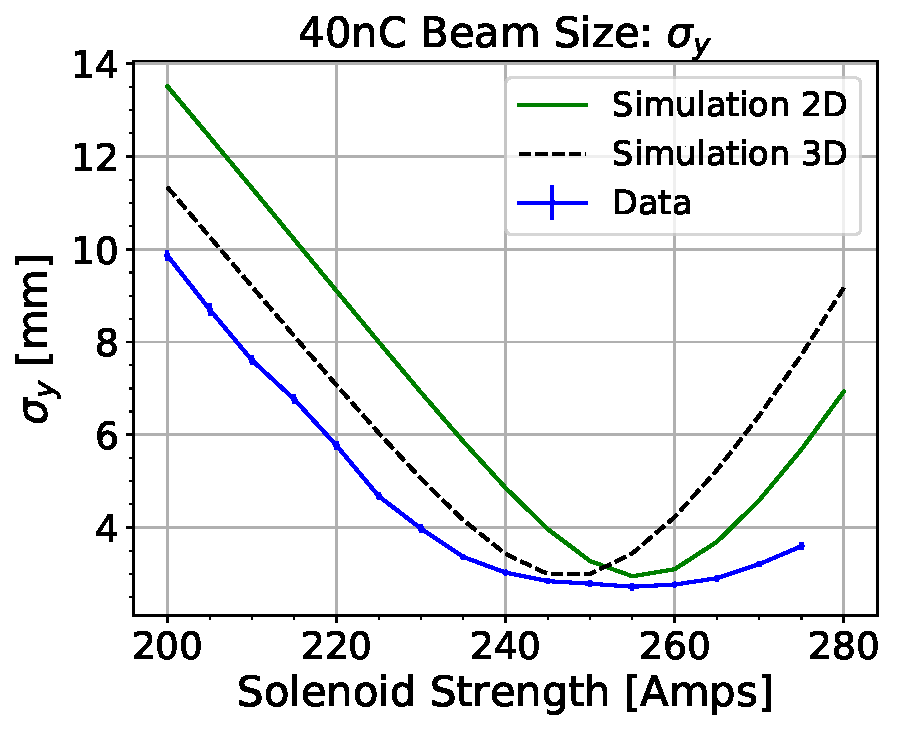
\includegraphics[width=1.0\linewidth]{/home/nicole/Documents/presentations/group_meetings/ybeamsizes_high_charge_sol_scan_10-17-2017}
		\end{minipage}
	\end{column}
	\begin{column}{0.4\textwidth}
		%\vspace{-9em}
		\begin{itemize}
			\item only charge fluctuations are considered in error bars
			\item Need to check laser profiles  
			\item Radius probably needs to be adjusted in simulations of high charge
		\end{itemize}
	\end{column}
\end{columns}
\end{frame}

\begin{frame}
\frametitle{BF Solenoid Scans}
\begin{columns}[T]
	\begin{column}{0.76\textwidth}
		\begin{minipage}{0.5\textheight}
			\includegraphics[width=1.0\linewidth]{/home/nicole/Documents/presentations/group_meetings/xbeamsizes_0pt7nC_BFsol_scan2}
			\includegraphics[width=1.0\linewidth]{/home/nicole/Documents/presentations/group_meetings/ybeamsizes_0pt7nC_BFsol_scan2}%
		\end{minipage}
		\begin{minipage}{0.5\textheight}
			\includegraphics[width=1.0\linewidth]{/home/nicole/Documents/presentations/group_meetings/xbeamsizes_1nC_BFsol_scan}
			\includegraphics[width=1.0\linewidth]{/home/nicole/Documents/presentations/group_meetings/ybeamsizes_1nC_BFsol_scan}
		\end{minipage}
	\end{column}
	\begin{column}{0.4\textwidth}
		%\vspace{-9em}
		\begin{itemize}
			\item Again, radius may need adjustment
			\item M=0 images were partly off screen, need to play with fit for these
		\end{itemize}
	\end{column}
\end{columns}
\end{frame}

\end{frame}
%%%%%%%%%%%%%%%%%%%%%%%%%%%%%%%%%%%%%%%%%%%%%%%%%%%%%%%%%%%%%%%%%%%%%%%%%%%%%%%%

%%%%%%%%%%%%%%%%%%%%%%%%%%%%%%%%%%%%%%%%%%%%%%%%%%%%%%%%%%%%%%%%%%%%%%%%%%%%%%%%



\begin{frame}
\frametitle{Sensitivity Analysis}

\vspace{-0.5em}
Reminder of why matching to simulations is important...
\centering
\includegraphics[width=0.8\textwidth]{/home/nicole/Documents/surrogatemodels/ml-ws-poster/awa-medium-o4/sensresults.pdf}
\end{frame}
%%%%%%%%%%%%%%%%%%%%%%%%%%%%%%%%%%%%%%%%%%%%%%%%%%%%%%%%%%%%%%%%%%%%%%%%%%%%%%%%
\begin{frame}
	\frametitle{Summary}
	\begin{itemize}
		\item 
		\begin{itemize}
			\item 
			\item 
			\item 
			\item 

		\end{itemize}
		\item 
		\item 
		
	\end{itemize}

	\vspace{1em}
	\centering
	\color{blue}\huge{Thanks for your attention!}

\end{frame}

%%%%%%%%%%%%%%%%%%%%%%%%%%%%%%%%%%%%%%%%%%%%%%%%%%%%%%%%%%%%%%%%%%%%%%%%%%%%%%%%
\end{document}
















